\section{Experiments and Evaluation}
We conduct several experiments for all four settings to evaluate the influence of order awareness and availability of dependency type information to the similarity prediction performance. In the following, we describe the dataset and the hyperparameter setting. Finally, we present the results and an analysis of errors.

\subsection{Dataset}
We use the SICK corpus\footnote{\url{http://alt.qcri.org/semeval2014/task1/index.php?id=data-and-tools}} \autocite{marelli_sick_2014} for model training and evaluation. The corpus consists of about approximately 10.000 pairs of English sentences based on the 8K ImageFlickr data set\footnote{\url{http://nlp.cs.illinois.edu/
HockenmaierGroup/data.html}} \autocite{hodosh_framing_2013} and the SemEval 2012 STS MSR-Video Description data set\footnote{\url{https://www.cs.york.ac.uk/semeval-2012/task6/index.php\%3Fid=data.html}} \autocite{agirre_semeval-2012_2012} that contain sentences describing the same picture or video. These sentences were linguistically normalized, so Named Entities and complex verb constructions are replaced or subordinates are turned into coordinates, for instance. Furthermore, they are manually expanded to generate candidate pairs that were labeled by 5 annotators with one to five point relatedness ratings that are averaged to produce a relatedness score. We rescaled the scores into the interval $[0.0, 1.0]$ to let them fit into our definition of a similarity measure. Table~\ref{tab:sick_examples} shows some examples of the dataset. The mean of the score for both train and test set is approximately $0.63$. The sentences have an average length of $9.6$ words and contain $2408$ different token types.  
%mean score: 0.63 * 4.0 + 1.0 = 3.53
\todo{AB:explain why SICK}

\begin{table*}[!htb]
\centering
  \begin{tabular}{p{0.4\textwidth}|p{0.4\textwidth}|c}
    sentence A & sentence B & score \\ \hline \hline
    A man in a shirt dyed purple is looking at a man in a black shirt who is doing a funny face & A man in a shirt dyed purple is looking at a man in a black shirt who is doing a face which looks funny & 1.0 \\ \hline
    A group of kids is playing in a yard and an old man is standing in the background & A group of boys in a yard is playing and a man is standing in the background & 0.875 \\ \hline
    A brown dog is attacking another animal in front of the man in pants & Two dogs are wrestling and hugging & 0.55 \\ \hline
    A woman is chopping an onion & A woman is washing her feet & 0.0
  \end{tabular}
  \caption{Example sentence pairs from SICK corpus with rescaled relatedness score ranging from $0.0$ (not related) to $1.0$ (maximal related).}
\label{tab:sick_examples}
\end{table*}

%\subsubsection{SICK}

%\subsubsection{PPDB}
%Our pre-training dataset is based on the phrasal part of the PPDB 2.0 dataset \autocite{pavlick_ppdb_2015}. We use a subset of 100,000 paraphrases and add an equal amount of negative samples by replacing for each pair the second paraphrase entry with a random phrase sampled uniformly\footnote{We also tried to sample according to the Jaccard similarity distribution of the original pairs, but this decreased the performance.} from all existing second pair entries. A similarity score of 1.0 is assigned to the original paraphrase pairs, the negative samples are scored with 0.0.

\subsection{Training and Hyperparameters}
We train the model in batches of 100 examples. The ADAM optimizer is initialized with a learning rate of 0.003. We apply gradient clipping by global norm as specified in \textcite{pascanu_difficulty_2012} with a threshold of 5.0 and use dropout \autocite{srivastava_dropout_2014} with a keep probability of 0.8 at the \ac{LSTM} and the \ac{FC} in the \ac{AVG} case to prevent from overfitting. We used a grid search at the train/dev set to find this parameter configuration. We applied 5-fold cross validation with regard to the train/dev split for every setting and repeated each experiment 10 times to achieve robust results.

\subsection{Results}
We measured performance using the Pearson correlation coefficient and \ac{MSE} between the predictions and gold scores. The mean Pearson correlation of all runs is about $0.839$ with a \ac{std} of $0.002$ and the mean \ac{MSE} is $0.024$ with std of $0.004$. The \ac{TF-IDF} baseline produces a Pearson score of $0.619$ and a \ac{MSE} of $0.082$. Thus, the regarded models achieve a mean \ac{MSE} performance gain of $+6.4\%$ with respect to the baseline. This performance lies in the range of the best system submitted for SemEval-2014 relatedness prediction task (MSE: $0.020$, Pearson's r: $0.828$), but stays below state of the art. Recent systems achieve MSE/Pearson's r scores of $0.016$/$0.87$ \autocite{he_multi-perspective_2015} or $0.014$/$0.88$ \autocite{mueller_siamese_2016}. We list the individual performances of the models examined in this work averaged over identical parameter settings in Table~\ref{tab:results}. Figure~\ref{fig:res_all} displays the \ac{MSE} and Pearson's r results for all parameter combinations as box plots\footnote{The boxes of all box plots show the \ac{IQR}, whiskers mark the $[1.5\times \text{IQR}, 3\times \text{IQR}]$ range and notches the  $10000\times$ bootstrapped confidence intervals.}. Note, that the y-axis is inverted for all box plots visualizing \ac{MSE} scores to show better performing scores above worse ones and to provide comparability with plots of Pearson scores. 
%# SICK_VERBADJNOUN_lemma	0.611	0.091		# TFIDF
%# SICK_ADJNOUN_lemma	0.558	0.111			# TFIDF
%# SICK_VERBADJNOUN_orth	0.568	0.106		# TFIDF
%# SICK_ADJNOUN_orth	0.542	0.119			# TFIDF

%\begin{figure}[htb!]
%  \centering
%  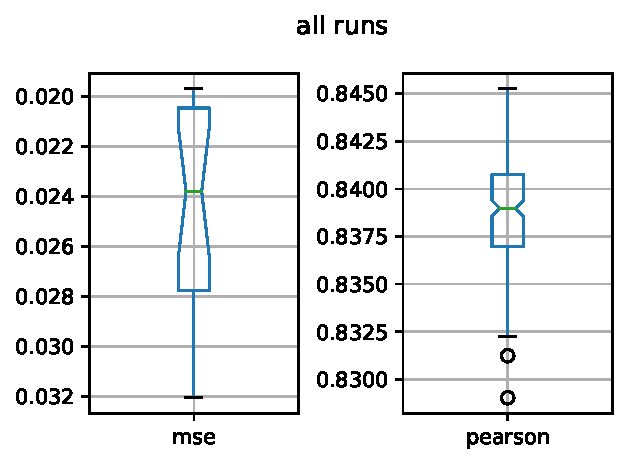
\includegraphics[width=0.9\textwidth]{results/fig_merged.pdf}
%  \caption{Overall model performance as Pearson correlation and MSE.}
%  \label{fig:res_merged}
%\end{figure}

%\begin{figure}[htb!]
%  \centering
%  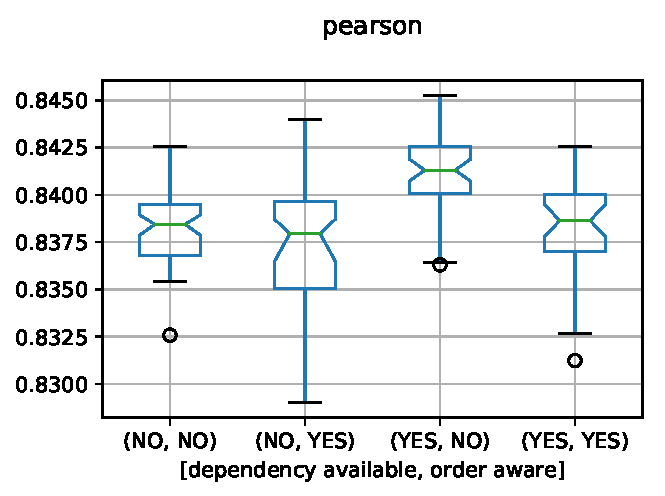
\includegraphics[width=0.9\textwidth]{results/fig_sep_pearson.pdf}
%  \caption{Pearson correlation scores for the different settings.}
%  \label{fig:res_sep_pearson}
%\end{figure}

%\begin{subtable}[c]{\textwidth}
%	\centering
\begin{table}[htb!]
  	\centering
  	%\begin{tabular}{|l|l|l|}
 \begin{tabularx}{\textwidth}{|X X|X|X|}
 %\begin{tabularx}{\textwidth}{|p{0.21\textwidth} p{0.15\textwidth}|X|X|} %{p{0.4\textwidth}|p{0.4\textwidth}|c}
		\hline
		dependency type & order aware & mse & pearson \\ \hline \hline
		NO & NO & 0.0284 & 0.8382 \\ 
		NO & YES & 0.0206 & 0.8375 \\
		YES & NO & 0.0274 & 0.8413 \\
		YES & YES & 0.0205 & 0.8383 \\ \hline \hline
		\multicolumn{2}{|l|}{TFIDF} & 0.0823 & 0.6189 \\ \hline
 \end{tabularx}
 %\captionsetup{width=0.9\linewidth}
 \caption{MSE and Pearson scores aggregated by setting.}
 \label{tab:results}
\end{table}
%	\vspace*{0.8 cm} \newline
	
  %\caption{Average \ac{MSE} and Pearson's r scores}
%\end{table}


\begin{figure}[htb!]
  \centering
  \textbf{Overall performance by setting}\par\medskip
  \begin{subfigure}{.5\textwidth}
    \centering
    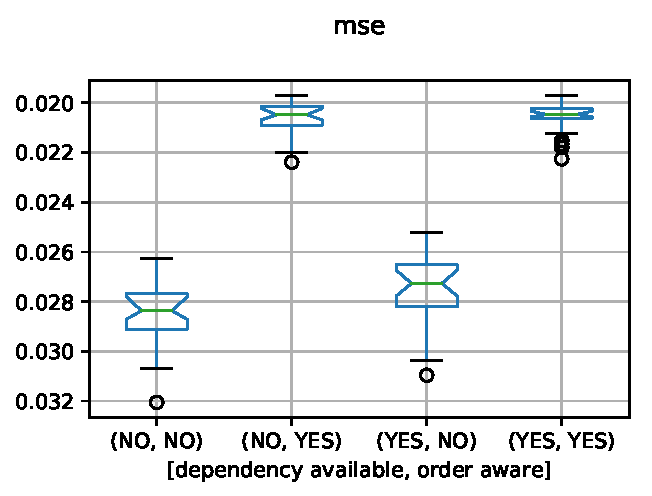
\includegraphics[width=1.\linewidth]{results/fig_sep_mse.pdf}
    \captionsetup{width=0.9\linewidth}
    %\caption{MSE for the different settings (inverted y-axis).}
  \end{subfigure}%
  \begin{subfigure}{.5\textwidth}
    \centering
    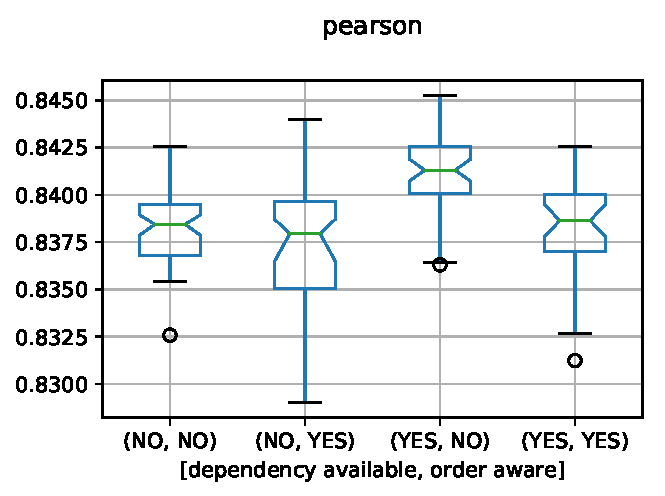
\includegraphics[width=1.\linewidth]{results/fig_sep_pearson.pdf}
    \captionsetup{width=0.9\linewidth}
    %\caption{Pearson's r for the different settings.}
  \end{subfigure}
  \caption{MSE (inverted y-axis) and Pearson's r for the different settings.}
  \label{fig:res_all}
\end{figure}

Adding \textbf{dependency types} improves the overall \ac{MSE} by $0.05\%$ and Pearson's r increases by $0.24\%$, whereby the former is not significant (p=0.336), but the later is ($p<0.0001$). Enabling the feature \textbf{order aware} results in a significant overall performance gain of $0.75\%$ in means of \ac{MSE} and a performance decrease of $-0.21\%$ with regard to Pearson's r ($p<0.0001$ for two-tailed t-test \todo{AB:ref?} in both cases). Table~\ref{tab:results_merged} shows the specific scores.

\begin{table}[htb!]
	\centering
	\begin{tabularx}{\textwidth}{|p{0.25\textwidth} p{0.15\textwidth}|X X|X X|} 
		%\begin{tabularx}{\textwidth}{|p{0.21\textwidth} X|X|X|} %{p{0.4\textwidth}|p{0.4\textwidth}|c}
		\hline
		parameter & enabled & mse & & pearson  & \\ \hline \hline
		dependency type & NO & 0.0245 & & 0.8378 & \\
		dependency type & YES & 0.0240 & $+0.05\%$* & 0.8398 & $+0.24$\% \\ \hline
		order aware & NO & 0.0279 &  & 0.8397 &  \\
		order aware & YES & 0.0206 & $+0.75\%$ & 0.8379 & $-0.21\%$ \\ \hline	   		
	\end{tabularx}
	%\captionsetup{width=0.9\linewidth}
	\caption{Scores aggregated by individual parameter assignment and percentage improvement when enabling the feature. The improvement marked with (*) is not significant.}
	\label{tab:results_merged}
\end{table}

Finding these contradictory results\todo{AB:with respect to the applied measure?}, we took a closer look at the deviations of the predicted relatedness scores from the gold scores. Figure~\ref{fig:fig_sorted_errors_sep} shows the deviations per setting ordered by gold score. It suggests that the averaging model (\texttt{order aware} = NO) strongly overestimates the relatedness score. Indeed, the mean deviation for all predictions in the averaging case ($+0.085$) is significant ($t < 0.0001$) higher when compared with non-averaging ($+0.019$). Because such a bias distorts the Pearson'r and \ac{MSE} was used as cost function while training, we focus at the \ac{MSE} measure for the rest of this work.

\begin{figure}[htb!]
	\centering
	\textbf{Deviations from gold score}\par\medskip
	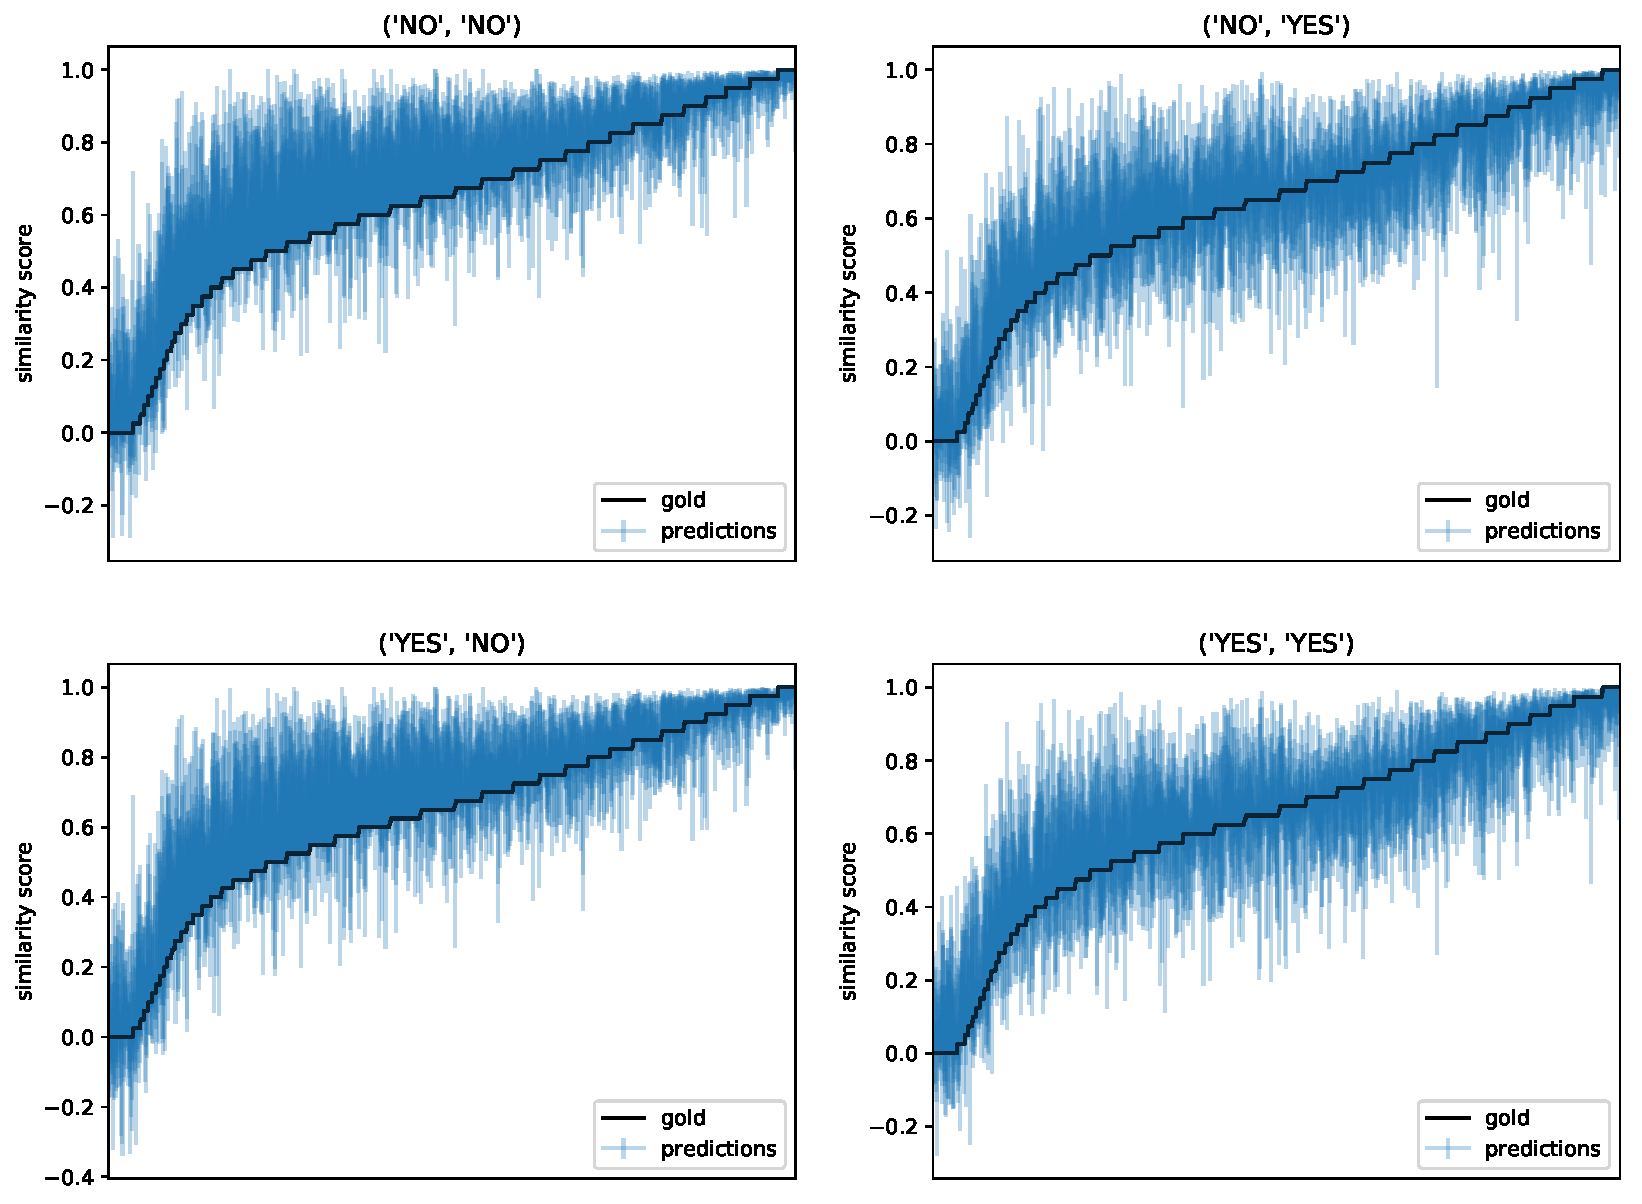
\includegraphics[width=1.\linewidth]{results/fig_sorted_errors_sep.pdf}
	\caption{Deviations of the predictions from gold similarity scores by setting (<dependency available>, <order aware>). The averaging models (order aware = NO; plots at the left) clearly overestimate.}
	\label{fig:fig_sorted_errors_sep}
\end{figure}

\subsubsection{Relation of Order Awareness and Dependency Types}
The specific performance in the examined settings suggests that the parameters Dependency Available and Order Aware are related. Figure~\ref{fig:fig_sep_cond} illustrates this by presenting the conditional impact of the parameters. Especially, the impact of Dependency Available seems to vary depending on activation of parameter Order Aware, whereas the opposite does not hold.\footnote{See table~\ref{tab:results} for the actual values.} This observation leads to the following question: What kind of useful information with respect to semantical awareness is encoded in dependency types? Precisely, we claim that

\begin{claim}
	Dependency types encode local context information that is useful to produce semantic aware compositional representations.
	%Useful context information is encoded in dependency types.
\end{claim}	

\begin{Proof}
	\begin{enumerate}
		\item Order Awareness as implemented within \ac{LSTM}s enable locally contextualized processing (see Section~\ref{subsec:order_aware_composition}). Thus, these models encode local context.
		\item As explained in section \ref{subsec:eval_semantic_awareness}, semantic awareness can be measured using the relatedness prediction task. Since enabling the parameter Order Aware significantly increases the prediction performance by $+0.8\%$ ($t < 0.0001$) shows that local context information is important to determine the meaning of a word in a specific textual utterance and to handle semantic aware composition.
		%As relatedness prediction is a general semantic task, it requires this information.
		\item Enabling the parameter Dependency Available significantly improves the model performance by $+0.1\%$ ($t < 0.001$), in the case of disabled Order Awareness, proving that dependency types indeed encode useful information.
		\item Since the order aware model does not perform significantly better with dependency type data ($t = 0.50$) it follows that this data does not encode extra useful information for order aware models.
		\item This strongly suggests that dependency types indeed encode local context.
	\end{enumerate}
\end{Proof}

\begin{figure}[htb!]
	\centering
	\textbf{Conditional parameter impact}\par\medskip
	\begin{subfigure}{.5\textwidth}
		\centering
		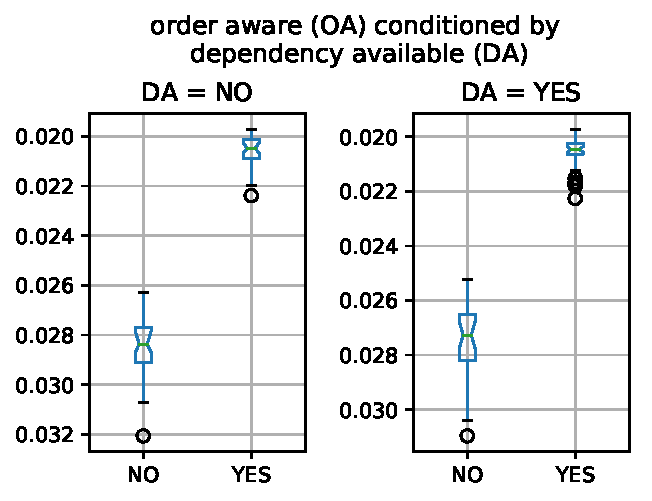
\includegraphics[width=1.\linewidth]{results/fig_sep_cond_order.pdf}
		%\captionsetup{width=0.9\linewidth}
		%\caption{Impact of parameter \textit{order aware} conditioned by enabled \textit{dependency available} parameter.}
	\end{subfigure}%
	\begin{subfigure}{.5\textwidth}
		\centering
		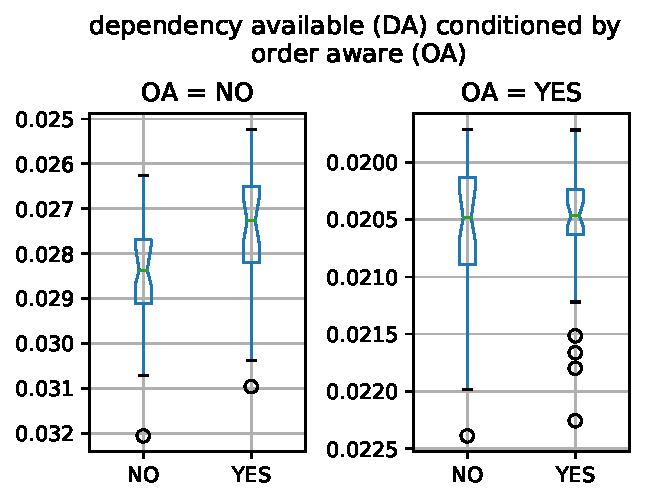
\includegraphics[width=1.\linewidth]{results/fig_sep_cond_dependency.pdf}
		%\captionsetup{width=0.9\linewidth}
		%\caption{Impact of parameter \textit{order aware} conditioned by disabled \textit{dependency available} parameter.}
		\captionsetup{width=0.9\linewidth}
		%\caption{Impact of parameter \textit{dependency available} conditioned by parameter \textit{dependency available}.}
	\end{subfigure}	
	\caption{Conditional parameter impact measured with MSE.}
	\label{fig:fig_sep_cond}
\end{figure}



%\begin{figure}[htb!]
%  \centering
%  \includegraphics[width=0.9\textwidth]{fig_sep_order.pdf}
%  \caption{Influence of order awareness measured with Pearson correlation and MSE.}
%  \label{fig:pearson_all_sep}
%\end{figure}

%\subsubsection{cosine vs. manhattan}
%\subsubsection{Dependency edge types}
%mean mse: 0.0245 -> 0.0240 =  -0.0005 \\
%mean pearson: 0.8378 -> 0.8398 =   0.0019 \\
%performance gain of 0,05\%*/0,31\% (mse/pearson) regarding TF-IDF baseline 

%*: not significant
%\begin{figure}[htb!]
%  \centering
%  \includegraphics[width=0.9\textwidth]{fig_sep_dep.pdf}
%  \caption{Influence of dependency edge type Information measured with Pearson correlation and MSE.}
%  \label{fig:pearson_all_sep}
%\end{figure}



%\subsubsection{Pretraining}

\subsubsection{Qualitative error analysis}



% Alternations / Diathese
%http://ling.uni-konstanz.de/pages/home/hautli/LR/verb-classes-levin.pdf
%http://ccl.pku.edu.cn/973_sem_spec/Sem_ling/English%20Verb%20Classes%20and%20Alternations%20A%20Preliminary%20Investigation.pdf

% pearson-correlation("('NO', 'NO') vs ('YES', 'NO') abs"; "score_jaccard") = -0.456
% > increasing overlap -> decreasing benefit of "dependency available" 
